\documentclass{article}

\usepackage[dvipdfmx]{graphicx}
\usepackage[margin=20truemm]{geometry}
\usepackage{indentfirst}

\usepackage{amsmath}
\usepackage{amsthm}

\title{WCA\_exportファイルの構造と統計処理}
\author{IronCuber333}
\date{}

\begin{document}
  \maketitle

  世界キューブ協会(World Cube Assosiation,WCA)のウェブサイトでは,スピードキューブの公式大会の結果などが掲載されている.結果などの統計情報の元となっているtsvファイルをダウンロードすることができる.これらの統計情報を解析するには各ファイルの内容を理解することが重要である.\par

  \section{tsvファイルの構造}

  tsvファイルは,各行が文字列がタブで区切られているファイル形式である.行と列があるため,Microsoft Excelなどで開くことができる.プログラムでこれを扱うため,以降行番号や列番号は$ 0 $を起点とする.つまり,最初の行は$ 0 $行目であり,以降$ 1 $行目,$ 2 $行目$ \cdots $と続く.\par
  とりわけ,WCAのファイルは,図\ref{figure:countries}などのように,0行目に項目の名前,1行目以降に各項目の内容が記述されてある.\par

  \section{各ファイルの内容}

  \subsection{WCA\_export\_Continentsファイル}

  大陸(地域)に関する情報がまとめられている.(図\ref{figure:continents},表\ref{table:continents})\par

  \begin{figure}[h]
    \centering
    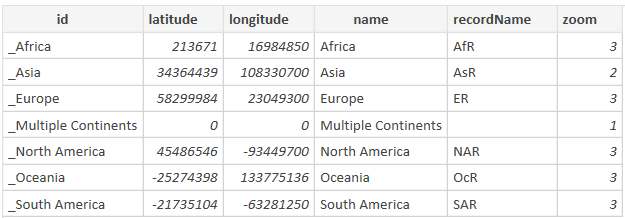
\includegraphics[height=24mm]{continents.png}
    \caption{WCA\_export\_Continentsファイルのプレビュー}
    \label{figure:continents}
  \end{figure}

  \begin{table}[h]
    \centering
    \caption{WCA\_export\_Continentsファイルの内容}
    \label{table:continents}
    \begin{tabular}{l|l|l}
      \hline
      列番号 & 項目名 & 内容 \\
      \hline \hline
      $ 0 $ & id & 大陸を識別するためのID. \\
      $ 1 $ & latitude & 大陸中心の緯度. \\
      $ 2 $ & longitude & 大陸中心の経度. \\
      $ 3 $ & name & 大陸名. \\
      $ 4 $ & recordName & 大陸記録の名前. \\
      $ 5 $ & zoom & 不明. \\
      \hline
    \end{tabular}
  \end{table}

  世界キューブ協会では,世界の各地域をアフリカ,アジア,ヨーロッパ,北アメリカ,オセアニア,南アメリカの$ 6 $つの大陸(地域)に区分している.Continentsファイルでは,これらの地域に加え,複数地域という区分も用意されている.\par

  \subsection{WCA\_export\_Countriesファイル}

  国に関する情報がまとめられている.(図\ref{figure:countries},表\ref{table:countries})\par

  \begin{figure}[h]
    \centering
    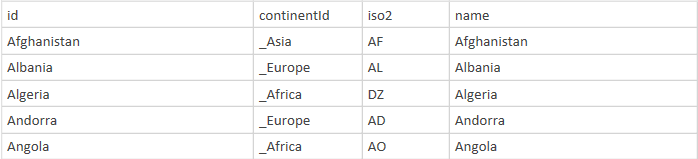
\includegraphics[height=18mm]{countries.png}
    \caption{WCA\_export\_Countriesファイルのプレビュー}
    \label{figure:countries}
  \end{figure}

  \begin{table}[h]
    \centering
    \caption{WCA\_export\_Countriesファイルの内容}
    \label{table:countries}
    \begin{tabular}{l|l|l}
      \hline
      列番号 & 項目名 & 内容 \\
      \hline \hline
      $ 0 $ & id & 国を識別するためのID. \\
      $ 1 $ & countinentId & 国が所属する大陸のID. \\
      $ 2 $ & iso2 & idと同様に,国を識別するためのID.この方式では,英字$ 2 $文字で表す. \\
      $ 3 $ & name & 国名. \\
      \hline
    \end{tabular}
  \end{table}

  世界キューブ協会では,各国の国内記録や国内ランキングも管理している.競技者の国籍や,大会の開催国を管理する上で国に関する情報は必要である.\par

  \subsection{WCA\_export\_eligible\_country\_iso2s\_for\_championshipファイル}

  上記の大陸区分とは異なる,国の集合体.(図\ref{figure:eligible},表\ref{table:eligible})\par

  \begin{figure}[h]
    \centering
    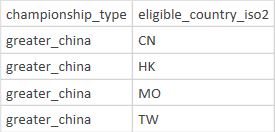
\includegraphics[height=15mm]{eligible.png}
    \caption{WCA\_export\_eligible\_country\_iso2s\_for\_championshipファイルのプレビュー}
    \label{figure:eligible}
  \end{figure}

  \begin{table}[h]
    \centering
    \caption{WCA\_export\_eligible\_country\_iso2s\_for\_championshipファイルの内容}
    \label{table:eligible}
    \begin{tabular}{l|l|l}
      \hline
      列番号 & 項目名 & 内容 \\
      \hline \hline
      $ 0 $ & championship\_type & 複数の国を扱うチャンピョンシップのタイプ. \\
      $ 1 $ & eligible\_country\_iso2 & 国のiso2(英字$ 2 $文字で表された国を識別するためのID). \\
      \hline
    \end{tabular}
  \end{table}

  チャンピョンシップ大会では,特定の地域の競技者の中からチャンピョンを決めることになっている.基本的には国別大会,大陸別大会,世界大会の$ 3 $種類であるが,greater\_chinaという形式のチャンピョンシップ大会では,中国,香港,マカオ,台湾の競技者の中からチャンピョンを決定する.\par

  \subsection{WCA\_export\_Eventsファイル}

  種目に関する情報がまとめられている.(図\ref{figure:events},表\ref{table:events})\par

  \begin{figure}[h]
    \centering
    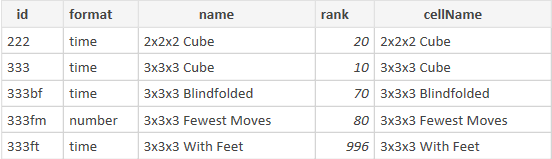
\includegraphics[height=18mm]{events.png}
    \caption{WCA\_export\_Eventsファイルのプレビュー}
    \label{figure:events}
  \end{figure}

  \begin{table}[h]
    \centering
    \caption{WCA\_export\_Eventsファイルの内容}
    \label{table:events}
    \begin{tabular}{l|l|l}
      \hline
      列番号 & 項目名 & 内容 \\
      \hline \hline
      $ 0 $ & id & 種目を識別するためのID. \\
      $ 1 $ & format & 記録のフォーマット.3x3x3 最小手数,3x3x3 複数目隠し特有のフォーマットがあるため. \\
      $ 2 $ & name & 種目名. \\
      $ 3 $ & rank & 種目の順番を決定するための数値.小さい順に3x3x3キューブ,2x2x2キューブ,$ \cdots $と続く. \\
      $ 4 $ & cellName & 種目名の略称.$ 2 $列目のnameと同様である. \\
      \hline
    \end{tabular}
  \end{table}

  世界キューブ協会にはいくつかの公式種目があり,これらの記録を認定している.記録のフォーマットはtime,number,multiの$ 3 $種類がある.最も一般的なものはtimeで,小数第$ 2 $位まで記録されたタイムを$ 100 $倍してint型で記録する方式である.numberは3x3x3 最小手数の単発記録の手数をそのままint型として記録する方式である.ただし,平均記録はtimeと同様に,小数第$ 2 $位まで記録された手数を$ 100 $倍してint型として記録されている.multiは3x3x3 複数目隠し特有のフォーマットである.3x3x3 複数目隠しでは,成功した個数,挑戦した個数,およびタイムが記録される.このとき,成功した個数から失敗した個数を引くことで求められる点数,タイム,失敗した個数の少なさという優先順位で順位がつけられる.これらを$ 1 $つのint型整数で表している.multiフォーマットの記録は$ 9 $桁の整数になっており,左から$ 1 $番目から$ 2 $番目が$ 99 $からポイントを引いたもの,$ 3 $番目から$ 7 $番目がタイム,$ 8 $番目から$ 9 $番目が失敗した個数を表している.いずれの形式も,$ 0 $は該当記録なし,$ -1 $はDNF(Did Not Finish),$ -2 $はDNS(Did Not Start)を表している.\par

  \subsection{WCA\_export\_Formatsファイル}

  試技のフォーマットに関する情報がまとめられている.(図\ref{figure:formats},表\ref{table:formats})\par

  \begin{figure}[h]
    \centering
    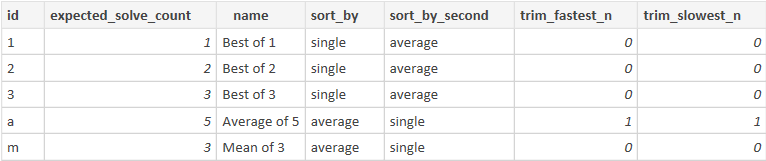
\includegraphics[height=18mm]{formats.png}
    \caption{WCA\_export\_Formatsファイルのプレビュー}
    \label{figure:formats}
  \end{figure}

  \begin{table}[h]
    \centering
    \caption{WCA\_export\_Formatsファイルの内容}
    \label{table:formats}
    \begin{tabular}{l|l|l}
      \hline
      列番号 & 項目名 & 内容 \\
      \hline \hline
      $ 0 $ & id & フォーマットを識別するためのID. \\
      $ 1 $ & expected\_solve\_count & 試技に含まれる単発記録の個数. \\
      $ 2 $ & name & 種目名. \\
      $ 3 $ & sort\_by & 順位を決定するために単発と平均のどちらを採用するか. \\
      $ 4 $ & sort\_by\_second & sort\_byが同じであった場合,こちらの指標で順位がつけられる. \\
      $ 5 $ & trim\_fastest\_n & 平均を計算する際,速い記録をいくつ除外するか. \\
      $ 6 $ & trim\_slowest\_n & 平均を計算する際,遅い記録をいくつ除外するか. \\
      \hline
    \end{tabular}
  \end{table}

  各種目の記録のフォーマットとは別に,試技のフォーマットもいくつか用意されている.Best of 1,Best of 2,Best of 3は最も良い単発記録で競う形式である.Average of 5は$ 5 $回の試技の中から最も良い記録と最も悪い記録を除いた$ 3 $つ平均値を競う形式である.Mean of 3は$ 3 $回の試技の平均値を競う形式である.\par

  \subsection{WCA\_export\_Competitionsファイル}

  大会に関する情報がまとめられている.(図\ref{figure:competitions1},図\ref{figure:competitions2},図\ref{figure:competitions3},表\ref{table:competitions})\par

  \begin{figure}[h]
    \centering
    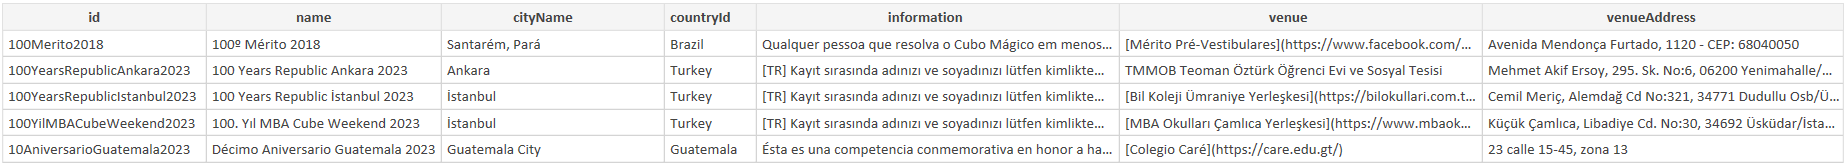
\includegraphics[height=18mm]{competitions1.png}
    \caption{WCA\_export\_Competitionsファイルのプレビュー$ 1 $}
    \label{figure:competitions1}
  \end{figure}
  \begin{figure}[h]
    \centering
    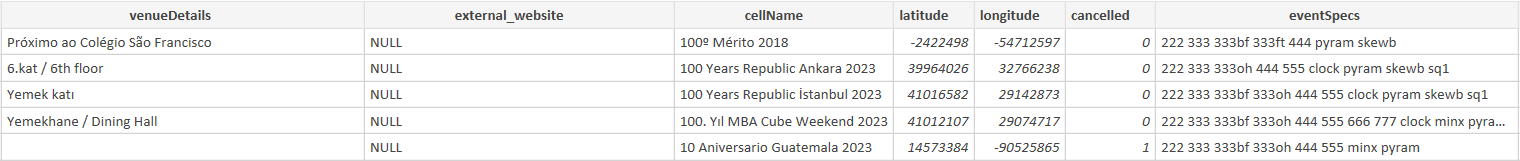
\includegraphics[height=18mm]{competitions2.png}
    \caption{WCA\_export\_Competitionsファイルのプレビュー$ 2 $}
    \label{figure:competitions2}
  \end{figure}
  \begin{figure}[h]
    \centering
    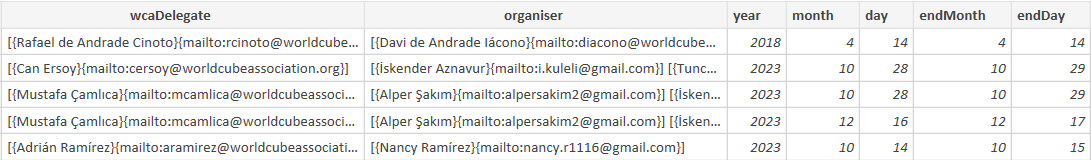
\includegraphics[height=18mm]{competitions3.png}
    \caption{WCA\_export\_Competitionsファイルのプレビュー$ 3 $}
    \label{figure:competitions3}
  \end{figure}

  \begin{table}[h]
    \centering
    \caption{WCA\_export\_Competitionsファイルの内容}
    \label{table:competitions}
    \begin{tabular}{l|l|l}
      \hline
      列番号 & 項目名 & 内容 \\
      \hline \hline
      $ 0 $ & id & 大会を識別するためのID. \\
      $ 1 $ & name & 大会名. \\
      $ 2 $ & cityName & 大会が開催される都市. \\
      $ 3 $ & countryId & 大会が開催される国のID. \\
      $ 4 $ & information & 大会の基本情報. \\
      $ 5 $ & venue & 大会会場の名前. \\
      $ 6 $ & venueName & 大会会場の住所. \\
      $ 7 $ & venueDetail & 大会会場の詳細.部屋など. \\
      $ 8 $ & external\_website & 大会の外部ウェブサイト. \\
      $ 9 $ & cellName & 大会の略称.大会名と同じ場合もある. \\
      $ 10 $ & latitude & 大会会場の緯度. \\
      $ 11 $ & longitude & 大会会場の経度. \\
      $ 12 $ & cancelled & 大会がキャンセルされたかどうか. \\
      $ 13 $ & eventSpecs & 開催された種目のID. \\
      $ 14 $ & wcaDelegate & 担当のWCA Delegate. \\
      $ 15 $ & organiser & 大会の実行委員. \\
      $ 16 $ & year & 大会の開催年. \\
      $ 17 $ & month & 大会の開催月. \\
      $ 18 $ & day & 大会の開催日. \\
      $ 19 $ & endMonth & 大会の終了月. \\
      $ 20 $ & endDay & 大会の終了日. \\
      \hline
    \end{tabular}
  \end{table}

  \subsection{WCA\_export\_championshipsファイル}

  大会の中でも,チャンピョンシップ大会に関する情報がまとめられている.(図\ref{figure:championships},表\ref{table:championships})\par

  \begin{figure}[h]
    \centering
    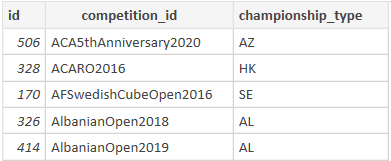
\includegraphics[height=18mm]{championships.png}
    \caption{WCA\_export\_championshipsファイルのプレビュー}
    \label{figure:championships}
  \end{figure}

  \begin{table}[h]
    \centering
    \caption{WCA\_export\_championshipsファイルの内容}
    \label{table:championships}
    \begin{tabular}{l|l|l}
      \hline
      列番号 & 項目名 & 内容 \\
      \hline \hline
      $ 0 $ & id & チャンピョンシップ大会を識別するためのID. \\
      $ 1 $ & competitionId & 大会のID. \\
      $ 2 $ & championship\_type & チャンピョンシップ大会のタイプ.世界大会,大陸別大会など. \\
      \hline
    \end{tabular}
  \end{table}

  チャンピョンシップ大会がいずれの地域の大会であるかを表している.国別大会の場合は国のiso2が,大陸別大会の場合は大陸IDが,世界大会の場合はworldがチャンピョンシップ大会のタイプとして割り当てられている.$ 1 $つの大会が複数のタイプのチャンピョンシップ大会を兼ねていることもある.\par

  \subsection{WCA\_export\_RoundTypesファイル}

  大会におけるラウンドに関する情報がまとめられている.(図\ref{figure:roundTypes},表\ref{table:roundTypes})\par

  \begin{figure}[h]
    \centering
    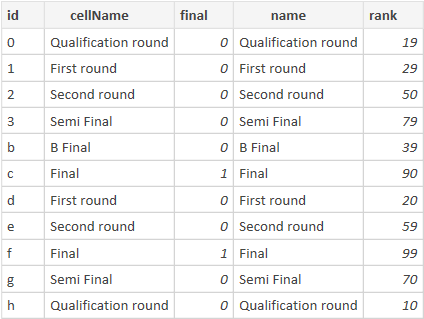
\includegraphics[height=36mm]{roundTypes.png}
    \caption{WCA\_export\_RoundTypesファイルのプレビュー}
    \label{figure:roundTypes}
  \end{figure}

  \begin{table}[h]
    \centering
    \caption{WCA\_export\_RoundTypesファイルの内容}
    \label{table:roundTypes}
    \begin{tabular}{l|l|l}
      \hline
      列番号 & 項目名 & 内容 \\
      \hline \hline
      $ 0 $ & id & ラウンドを識別するためのID. \\
      $ 1 $ & cellName & ラウンド名の略称.$ 3 $列目のnameと同様である. \\
      $ 2 $ & final & 決勝かどうか. \\
      $ 3 $ & name & ラウンド名. \\
      $ 4 $ & rank & 種目の順番を決定するための数値. \\
      \hline
    \end{tabular}
  \end{table}

  ラウンドの種類については,過去に様々な方式が採用されていた経緯もあり,様々な種類が存在している.\par

  \subsection{WCA\_export\_Scramblesファイル}

  スクランブルに関する情報がまとめられている.(図\ref{figure:scrambles},表\ref{table:scrambles})\par

  \begin{figure}[h]
    \centering
    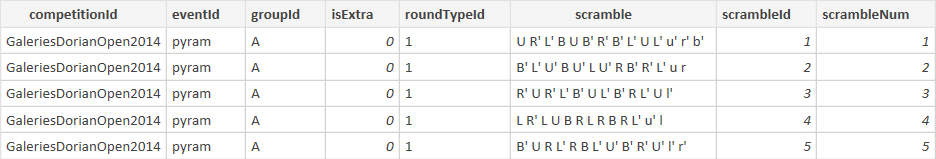
\includegraphics[height=18mm]{scrambles.png}
    \caption{WCA\_export\_Scramblesファイルのプレビュー}
    \label{figure:scrambles}
  \end{figure}

  \begin{table}[h]
    \centering
    \caption{WCA\_export\_Scramblesファイルの内容}
    \label{table:scrambles}
    \begin{tabular}{l|l|l}
      \hline
      列番号 & 項目名 & 内容 \\
      \hline \hline
      $ 0 $ & competitionId & 大会ID. \\
      $ 1 $ & eventId & 種目ID. \\
      $ 2 $ & groupId & グループID. \\
      $ 3 $ & isExtra & エクストラかどうか. \\
      $ 4 $ & roundTypeId & ラウンドID. \\
      $ 5 $ & scramble & スクランブル. \\
      $ 6 $ & scrambleId & スクランブルを識別するためのID. \\
      $ 7 $ & scrambleNum & スクランブル番号. \\
      \hline
    \end{tabular}
  \end{table}

  \subsection{WCA\_export\_Resultsファイル}

  結果に関する情報がまとめられている.(図\ref{figure:results},表\ref{table:results})\par

  \begin{figure}[h]
    \centering
    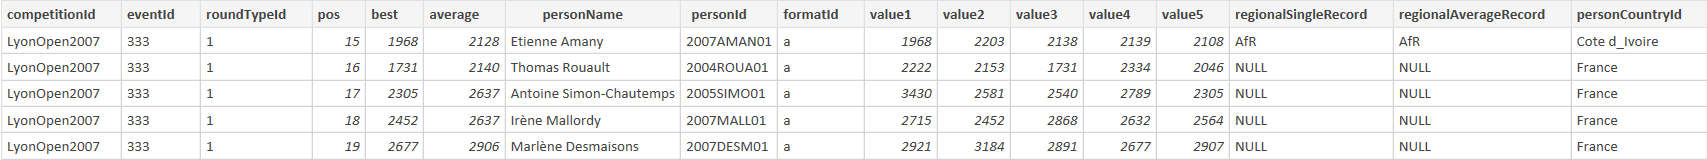
\includegraphics[height=18mm]{results.png}
    \caption{WCA\_export\_Resultsファイルのプレビュー}
    \label{figure:results}
  \end{figure}

  \begin{table}[h]
    \centering
    \caption{WCA\_export\_Resultsファイルの内容}
    \label{table:results}
    \begin{tabular}{l|l|l}
      \hline
      列番号 & 項目名 & 内容 \\
      \hline \hline
      $ 0 $ & competitionId & 大会ID. \\
      $ 1 $ & eventId & 種目ID. \\
      $ 2 $ & roundTypeId & ラウンドID. \\
      $ 3 $ & pos & 大会内順位. \\
      $ 4 $ & best & 単発ベスト記録. \\
      $ 5 $ & average & 平均記録. \\
      $ 6 $ & personName & 競技者名. \\
      $ 7 $ & personId & 競技者ID. \\
      $ 8 $ & formatId & フォーマットID. \\
      $ 9 $ & value1 & $ 1 $試技目の記録. \\
      $ 10 $ & value2 & $ 2 $試技目の記録. \\
      $ 11 $ & value3 & $ 3 $試技目の記録. \\
      $ 12 $ & value4 & $ 4 $試技目の記録. \\
      $ 13 $ & value5 & $ 5 $試技目の記録. \\
      $ 14 $ & regionalSingleRecord & 単発の地域記録. \\
      $ 15 $ & regionalAverageRecord & 平均の地域記録. \\
      $ 16 $ & personCountryId & 競技者の国のID. \\
      \hline
    \end{tabular}
  \end{table}

  大会結果は,$ 1 $回から$ 5 $回の試技を$ 1 $ラウンドの結果としてまとめて扱われる.\par

  \subsection{WCA\_export\_Personsファイル}

  競技者に関する情報がまとめられている.(図\ref{figure:persons},表\ref{table:persons})\par

  \begin{figure}[h]
    \centering
    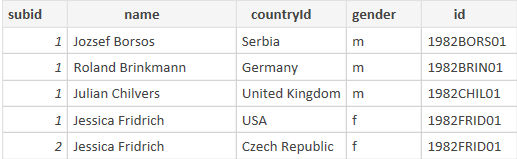
\includegraphics[height=18mm]{persons.png}
    \caption{WCA\_export\_Personsファイルのプレビュー}
    \label{figure:persons}
  \end{figure}

  \begin{table}[h]
    \centering
    \caption{WCA\_export\_Personsファイルの内容}
    \label{table:persons}
    \begin{tabular}{l|l|l}
      \hline
      列番号 & 項目名 & 内容 \\
      \hline \hline
      $ 0 $ & subid & サブとなるID.国籍や名前を変更した競技者は,複数のsub IDをもつ. \\
      $ 1 $ & name & 競技者名. \\
      $ 2 $ & countryId & 競技者の国籍のID. \\
      $ 3 $ & gender & 競技者の性別. \\
      $ 4 $ & id & 競技者を識別するためのID.WCA IDともよばれる. \\
      \hline
    \end{tabular}
  \end{table}

  競技者に対して,WCA IDが割り振られている.国籍や名前が途中で変わる場合もあるが,そのような場合は異なるsub IDとして管理している.国籍が途中で変わった場合でも,記録を出した時の国籍の国の記録として扱われる.\par

  \subsection{WCA\_export\_RanksSingleファイル}

  単発記録ランキングに関する情報がまとめられている.(図\ref{figure:ranksSingle},表\ref{table:ranksSingle})\par

  \begin{figure}[h]
    \centering
    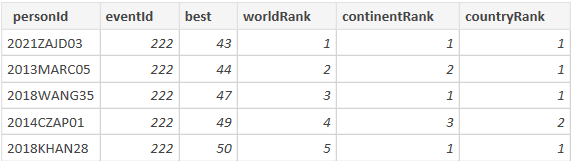
\includegraphics[height=18mm]{ranksSingle.png}
    \caption{WCA\_export\_RanksSingleファイルのプレビュー}
    \label{figure:ranksSingle}
  \end{figure}

  \begin{table}[h]
    \centering
    \caption{WCA\_export\_RanksSingleファイルの内容}
    \label{table:ranksSingle}
    \begin{tabular}{l|l|l}
      \hline
      列番号 & 項目名 & 内容 \\
      \hline \hline
      $ 0 $ & personId & 競技者ID. \\
      $ 1 $ & eventId & 種目ID. \\
      $ 2 $ & best & 記録. \\
      $ 3 $ & worldRank & 世界ランキング. \\
      $ 4 $ & continentRank & 大陸ランキング. \\
      $ 5 $ & countryRank & 国内ランキング. \\
      \hline
    \end{tabular}
  \end{table}
	
  \subsection{WCA\_export\_RanksAverageファイル}

  平均記録ランキングに関する情報がまとめられている.(図\ref{figure:ranksAverage},表\ref{table:ranksAverage})\par

  \begin{figure}[h]
    \centering
    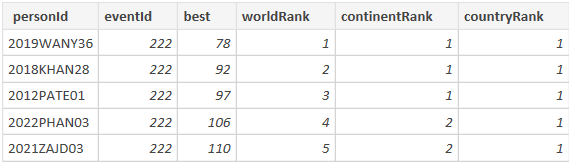
\includegraphics[height=18mm]{ranksAverage.png}
    \caption{WCA\_export\_RanksAverageファイルのプレビュー}
    \label{figure:ranksAverage}
  \end{figure}

  \begin{table}[h]
    \centering
    \caption{WCA\_export\_RanksAverageファイルの内容}
    \label{table:ranksAverage}
    \begin{tabular}{l|l|l}
      \hline
      列番号 & 項目名 & 内容 \\
      \hline \hline
      $ 0 $ & personId & 競技者ID. \\
      $ 1 $ & eventId & 種目ID. \\
      $ 2 $ & best & 記録. \\
      $ 3 $ & worldRank & 世界ランキング. \\
      $ 4 $ & continentRank & 大陸ランキング. \\
      $ 5 $ & countryRank & 国内ランキング. \\
      \hline
    \end{tabular}
  \end{table}

\end{document}